\chapter{Proceso de Selección, Transformación y Carga}
Como primer paso para el desarrollo del proyecto, teniendo en cuenta las fases de la metodología de descubrimiento del conocimiento \cite{key-50}, se debió proceder a la preparación de los datos, esto es más conocido como proceso de “Extracción, Transformación y Carga” (ETL, por sus siglas en ingles). Durante esta fase se trabajó en homogeneizar la información contenida en las bases de datos fuente. Se analizó cual era la mejor forma de estandarizarlos y la manera de almacenarlos para posteriormente usarlos en el procesamiento de los algoritmos de descubrimiento del conocimiento.
\section{Selección}
Las fuentes de información, donde se contenían los datos necesarios para la creación del clasificador, fueron de fácil recolección, ya que estas son suministradas directamente por el ICFES de manera libre.
El servicio brindado por el ICFES para el uso de estas bases de datos para promover la investigación ayuda a que se puedan realizar trabajos como este con el fin de determinar anomalías, conductas, mejoras, etc. sobre la calidad de la educación en Colombia.

La información recolectada estaba constituida por 24 bases de datos, que contenían información de cada uno de los exámenes aplicados a lo largo de 12 años desde el año 2000 hasta el 2011 (Actualmente la información del año 2012 ya se encuentra disponible, pero al momento de realizar este proceso de ETL no lo estaba, así que no se tomó como insumo para la construcción de los clasificadores), durante cada año se realizan 2 pruebas Saber 11\degree. La cantidad de registros almacenados en estas 24 bases de datos se encontraba alrededor de 5’700.000.

Las bases de datos fueron obtenidas en formato Access, un tipo de archivo que se utiliza para administrar bases de datos y pertenece a Microsoft. Para su primer procesamiento se decidió transportar la información a tablas administradas por el motor de bases de datos MySQL\footnote{\url{http://www.mysql.com/}}, esto se hizo, porque para la posterior transformación de los datos, los scripts de procesamiento se construyeron usando el lenguaje de programación Python\footnote{\url{http://www.python.org/}} y este tiene mejor soporte a la hora de conectarse con bases de datos MySQL.
\section{Transformación}
Teniendo la información recolectada se procedió a trasformar los datos obtenidos.

Esta transformación consta de estandarizar el formato en que son presentados los datos para su procesamiento, una coherencia entre el formato de presentación de los datos mejora la calidad de los resultados obtenidos, ya que estos tienen un valor de representación específico para cada caso que se puede presentar con cierto atributo, en caso de que para un atributo existan varios valores para indicar la misma situación o que para varias situaciones exista solo un valor valido, afecta la precisión con la que pueden trabajar los clasificadores.

Para la transformación del formato de los datos se utilizó como guía el diccionario de datos suministrado por el ICFES\footnote{\url{ftp://ftp.icfes.gov.co/SABER11/SB11-Diccionario_de_Datos-v1-6.pdf}}, en donde se muestra el historial de cómo se registró la información en las respectivas bases de datos. En este diccionario de puede apreciar la relación de las campos indagados, el año en que se registró y los valores con los que se registraba en cada año.

Los datos transformados y las modificaciones aplicadas se presentan a continuación: 
\begin{itemize}
\item Atributo COLE\_INST\_VLR\_PENSION indica con un código el valor mensual que pagó o paga el evaluado actualmente de pensión en el colegio.  Este atributo está presente en las 24 bases de datos, pero presenta variación en el formato de presentación, la tabla \ref{tab:cuadro2} muestra esta variación.

\begin{table}[!htb]
\centering
\begin{tabular}{|p{1.5cm}|p{2cm}|p{1.5cm}|p{2cm}|p{1.5cm}|p{2cm}|p{1.5cm}|p{2cm}|}
\hline
	\rowcolor[gray]{0.9} 
	\multicolumn{2}{|c|}{
	\textbf{Periodo 2000-2004}} &
	\multicolumn{2}{|c|}{
	\textbf{Periodo 2005-2007}} &
	\multicolumn{2}{|c|}{
	\textbf{Periodo 2008}} &
	\multicolumn{2}{|c|}{
	\textbf{Periodo 2009-2011}}\\
\hline
	\rowcolor[gray]{0.5}
	Código & Valor &
	Código & Valor &
	Código & Valor &
	Código & Valor \\
\hline
1 & No paga & 0 & No paga & 0 & No paga & 0 & No paga \\
\hline
2 & Menos de \$30.000 & 1 & Menos de \$33.000 & 8 & Menos de \$90.000 & 8 & Menos de \$87.000\\
\hline
3 & Entre \$30.000 y \$50.000 & 2 & Entre \$33.000 y menos de \$50.000 & 9 & Entre \$90.000 y menos de \$120.000 & 9 & Entre \$87.000 y menos de \$120.000\\
\hline
4 & Entre \$50.000 y menos de \$70.000 & 3 & Entre \$50.000 y menos de \$70.000 & 10 & Entre \$120.000 y menos de \$150.000 & 10 & Entre \$120.000 y menos de \$150.000\\
\hline
5 & Entre \$70.000 y menos de \$100.000 & 4 & Entre \$70.000 y menos de \$100.000 & 11 & Entre \$150.000 y menos de \$250.000 & 11 & Entre \$150.000 y menos de \$250.000\\
\hline
6 & Entre \$100.000 y menos de \$150.000 & 5 & Entre \$100.000 y menos de \$150.000 & 12 & \$250.000 o más & 12 & \$250.000 o más\\
\hline
7 & Entre \$150.000 y menos de \$250.000 & 6 & Entre \$150.000 y menos de \$250.000 & & & &\\
\hline
8 & Más de \$250.000 & 7 & Más de \$250.000 & & & &\\
\hline
\end{tabular}
\caption{Variación de la representación del atributo COLE\_INST\_VLR\_PENSION en las bases de datos.}
\label{tab:cuadro2}
\end{table}
Al analizar la variación en la representación del dato se puede notar que a medida que pasa el tiempo los rangos de especificación del valor de la pensión se han ido disminuyendo. Pero se pueden visualizar 3 rangos que son constantes ``No paga'', ``Entre \$150.000 y menos de \$250.000'' y ``\$250.000 o más'', por lo tanto siempre existió un valor que representara estos 3 niveles.

El problema aparece al momento de querer encontrar similitudes entre los rangos intermedios, se encuentra una representación de los datos casi igual entre el primer periodo con el segundo periodo  y entre el tercer periodo con el cuarto periodo.  Al momento de tomar la decisión se tuvo en cuenta cual transformación causaría una mejor perdida en la calidad de la información, por lo tanto se decidió dejar la representación utilizada en el periodo 2005-2007, ya que al momento de transformar los datos se mantiene una mayor especificidad, la cual no se mantendría si se hubieran tomado los valores de alguno de los últimos periodos.

Las transformaciones que tomaron los valores de los otros periodos se muestran en la tabla \ref{tab:cuadro3}.

\begin{table}[!htb]
\centering
\begin{tabular}{|p{2cm}|p{2cm}|p{2cm}|p{2cm}|p{2cm}|p{2cm}|}
\hline
	\rowcolor[gray]{0.9} 
	\multicolumn{2}{|c|}{
	\textbf{Periodo 2000-2004}} &
	\multicolumn{2}{|c|}{
	\textbf{Periodo 2008}} &
	\multicolumn{2}{|c|}{
	\textbf{Periodo 2009-2011}}\\
\hline
	\rowcolor[gray]{0.5}
	Código Anterior & Nuevo Código &
	Código Anterior & Nuevo Código &
	Código Anterior & Nuevo Código\\
\hline
1 & 0 & 0 & 0 & 0 & 0 \\
\hline
2 & 1 &  8 & 3 & 8 & 3\\
\hline
3 & 2 & 9 & 4 & 9 & 4\\
\hline
4 & 3 & 10 & 5 & 10 & 5\\
\hline
5 & 4 & 11 & 6 & 11 & 6\\
\hline
6 & 5 & 12 & 7 & 12 & 7\\
\hline
7 & 6 & & & & \\
\hline
8 & 7 & & & &\\
\hline
\end{tabular}
\caption{Transformación del atributo COLE\_INST\_VLR\_PENSION para ser registrado en el nuevo almacenamiento de datos.}
\label{tab:cuadro3}
\end{table}
\item Atributo ECON\_SN\_COMPUTADOR indica si el evaluado tiene o no tiene computador en la casa, en el años 2008 se preguntó en conjunto si la persona tenia servicio de internet y la cantidad de computadores que tenía. La variación de la representación de este atributo se presenta en la tabla \ref{tab:cuadro4}.

\begin{table}[!htb]
\centering
\begin{tabular}{|p{2cm}|p{2cm}|p{2cm}|p{2cm}|p{2cm}|p{2cm}|}
\hline
	\rowcolor[gray]{0.9} 
	\multicolumn{2}{|c|}{
	\textbf{Periodo 2008-I}} &
	\multicolumn{2}{|c|}{
	\textbf{Periodo 2008-II}} &
	\multicolumn{2}{|c|}{
	\textbf{Periodo 2009-2011}}\\
\hline
	\rowcolor[gray]{0.5}
	Código & Valor &
	Código & Valor &
	Código & Valor\\
\hline
0 & No & 0 & No & 0 & No \\
\hline
1 & Sí, con internet & 3 & Uno & 3 & Sí\\
\hline
2 & Sí, sin internet & 4 & Dos o más &  & \\
\hline
\end{tabular}
\caption{Variación de la representación del atributo ECON\_SN\_COMPUTADOR en las bases de datos.}
\label{tab:cuadro4}
\end{table}
El análisis de las representaciones deja visualizar que el factor importante de la información es conocer si el estudiante posee o no computador, por lo tanto los valores que se deciden dejar para que representen este valor en el nuevo almacenamiento de datos, solo deben indicar si la respuesta fue Sí o No, esta situación solo se encontraba en el último periodo, por lo tanto fue esta representación la que se decidió preservar. Las transformaciones aplicadas a los otros periodos se muestran en la tabla \ref{tab:cuadro5}.

\begin{table}[!htb]
\centering
\begin{tabular}{|p{2cm}|p{2cm}|p{2cm}|p{2cm}|}
\hline
	\rowcolor[gray]{0.9} 
	\multicolumn{2}{|c|}{
	\textbf{Periodo 2008-I}} &
	\multicolumn{2}{|c|}{
	\textbf{Periodo 2008-II}}\\
\hline
	\rowcolor[gray]{0.5}
	Código Anterior & Nuevo Código &
	Código Anterior & Nuevo Código \\
\hline
0 & 0 & 0 & 0  \\
\hline
1 & 3 & 3 & 3 \\
\hline
2 & 3 & 4 & 3 \\
\hline
\end{tabular}
\caption{Transformación del atributo ECON\_SN\_COMPUTADOR para ser registrado en el nuevo almacenamiento de datos.}
\label{tab:cuadro5}
\end{table}
\item Atributos: \begin{itemize} \item ESTU\_NACIMIENTO\_ANNO \item ESTU\_NACIMIENTO\_DIA \item ESTU\_NACIMIENTO\_MES \end{itemize} representan la fecha de nacimiento del estudiante. Estos 3 atributos tendrían un mayor significado si se presenta como ESTU\_EDAD, por lo tanto se realizó la transformación de estos para almacenar el valor numérico de la edad del estudiante.\\
La transformación se realizó calculando la fecha de presentación de examen con estos valores registrados, como la fecha exacta de los exámenes es desconocida, no se puede dar un 100\% de garantía de que todas las edades fueron correctamente registradas pero el rango de error no es mayor a un mes y esto es solo aplicable a los estudiantes que nacieron en los meses de abril o septiembre, esto es porque aunque no se tenga clara la fecha exacta de aplicación del examen si es conocido que el primer examen del año se realiza en abril y el segundo en septiembre.

Por ejemplo si un evaluado nació el 15 septiembre de 1995 y presentó el segundo examen del año 2011,  se calcula que este estudiante tiene una edad de 16 años, pero desconocemos el día en que se realizó el examen, si fue antes del día 15, entonces el cálculo de la edad es erróneo pero solo por unos pocos días, pero si se realizó después del día 15, entonces el cálculo es correcto.

Como se puede apreciar, a pesar de no existir una precisión del 100\% con todas las edades registradas, si se puede confiar en que en la gran mayoría de los casos estas son exactas y las que no lo son, tiene un error de pocos días.
\item Atributo ESTU\_TRABAJA indica si la persona trabaja, si el trabajo es remunerado y la cantidad de tiempo que dedica a trabajar. También presenta variaciones en sus registros, estas variaciones se presentan en la tabla \ref{tab:cuadro6}.

\begin{table}[!htb]
\centering
\begin{tabular}{|p{1.5cm}|p{2.5cm}|p{1.5cm}|p{10cm}|}
\hline
	\rowcolor[gray]{0.9} 
	\multicolumn{2}{|c|}{
	\textbf{Periodo 2000-2004I}} &
	\multicolumn{2}{|c|}{
	\textbf{Periodo 2008-2011}}\\
\hline
	\rowcolor[gray]{0.5}
	Código  & Valor &
	Código  & Valor \\
\hline
N & No & 0 & No  \\
\hline
S & Sí & 1 & Si, con remuneración en dinero y/o especie \\
\hline
 &  & 2 & Si, como ayudante sin remuneración \\
 \hline
 &  & 3 & Si, para contribuir a pagar su matrícula y/o los gastos del hogar \\
\hline
 &  & 4 & Si, por ser práctica obligatoria del programa de estudios \\
\hline
 &  & 5 & Si, para adquirir experiencia y/o recursos para sus gastos personales \\
\hline
 &  & 6 & Si, menos de 20 horas a la semana \\
\hline
 &  & 7 & Si, 20 horas o más a la semana \\ 
\hline
\end{tabular}
\caption{Variación de la representación del atributo ESTU\_TRABAJA en las bases de datos.}
\label{tab:cuadro6}
\end{table}
Al analizar la variación de la representación se observó que si se conservaban los valores de representación del segundo periodo era muy difícil encontrar un valor concordarte para el ``Sí'' del primer periodo, mientras que si se decidía conservar los valores de representación del primer periodo, todos los valores del segundo periodo tendrían una correspondencia en la transformación. Por lo tanto se decidió conservar la representación del primer periodo.

La transformación por lo tanto fue, el valor 0 se convirtió en ``N'' y los demás valores numéricos se convirtieron en ``S''.
\item Atributos FAMI\_COD\_EDUCA\_MADRE y FAMI\_COD\_EDUCA\_PADRE representa el nivel de educación de los padres, presentan 
variaciones en su representación. Las variaciones se presentan en la tabla \ref{tab:cuadro7}.

\begin{table}[!htb]
\centering
\begin{tabular}{|p{1.5cm}|p{6.5cm}|p{1.5cm}|p{6.5cm}|}
\hline
	\rowcolor[gray]{0.9} 
	\multicolumn{2}{|c|}{
	\textbf{Periodo 2000-2004I}} &
	\multicolumn{2}{|c|}{
	\textbf{Periodo 2008-2011}}\\
\hline
	\rowcolor[gray]{0.5}
	Código  & Valor &
	Código  & Valor \\
\hline
0 & Ninguno & 0 & Ninguno\\
\hline
1 & No tuvo Escuela & 9 & Primaria Incompleta\\
\hline
2 & Preescolar & 10 & Primaria Completa\\
\hline
3 & Básica Primaria & 11 & Secundaria (bachillerato) Incompleta\\
\hline
4 & Básica Secundaria & 12 & Secundaria (bachillerato) Completa\\
\hline
5 & Media Vocacional & 13 & Educación técnica o tecnológica incompleta\\
\hline
6 & Tecnológico o Técnico & 14 & Educación técnica o tecnológica Completa\\
\hline
7 & Universitario & 15 & Educación Profesional Incompleta\\ 
\hline
8 & Postgrado & 16 & Educación Profesional Completa\\
\hline
& & 17 & Postgrado\\
\hline
& & 99 & No sabe\\
\hline
\end{tabular}
\caption{Variación de la representación de los atributos FAMI\_COD\_EDUCA\_MADRE y FAMI\_COD\_EDUCA\_PADRE en las bases de datos.}
\label{tab:cuadro7}
\end{table}
Se observó que en el segundo periodo existe una mayor precisión sobre los datos almacenados, si se trasladan estos al primer periodo, se puede perder información importante, por lo tanto se decidió  transformar los valores del primer periodo a los del segundo. Sin embargo del primer periodo, los valores ``1'', ``2'' y ``5'' no tienen correspondencia en el segundo periodo, por lo tanto estos se conservaron sin modificación alguna. Los nuevos valores de representación se pueden observar en la tabla \ref{tab:cuadro8}.

\begin{table}[!htb]
\centering
\begin{tabular}{|p{2cm}|p{2cm}|}
\hline
	\rowcolor[gray]{0.9} 
	\multicolumn{2}{|c|}{
	\textbf{Periodo 2000-2004I}}\\
\hline
	\rowcolor[gray]{0.5}
	Código Anterior & Nuevo Código\\
\hline
0 & 0  \\
\hline
1 & 1  \\
\hline
2 & 2  \\
\hline
3 & 10  \\
\hline
4 & 12 \\
\hline
5 & 5 \\
\hline
6 & 14  \\
\hline
7 & 16 \\
\hline
8 & 17 \\
\hline
\end{tabular}
\caption{Transformación de los atributos FAMI\_COD\_EDUCA\_MADRE y FAMI\_COD\_EDUCA\_PADRE para ser registrados en el nuevo almacenamiento de datos.}
\label{tab:cuadro8}
\end{table}
\item Atributo FAMI\_COD\_OCUP\_MADRE y FAMI\_COD\_OCUP\_PADRE representan la actividad a la que se dedican los padres del evaluado. Presentan variaciones en su representación. Estas variaciones son mostradas en la tabla \ref{tab:cuadro9}.

\begin{table}[!htb]
\centering
\begin{tabular}{|p{1.5cm}|p{6.5cm}|p{1.5cm}|p{6.5cm}|}
\hline
	\rowcolor[gray]{0.9} 
	\multicolumn{2}{|c|}{
	\textbf{Periodo 2000-2004I}} &
	\multicolumn{2}{|c|}{
	\textbf{Periodo 2008-2011}}\\
\hline
	\rowcolor[gray]{0.5}
	Código  & Valor &
	Código  & Valor \\
\hline
0 & Fallecidos (solo se preguntó esta opción en 2000) & 13 & Empresario(a)\\
\hline
1 & Empresarios & 14 & Pequeño empresario(a)\\
\hline
2 & Administradores o gerentes & 15 & Empleado con cargo como director(a) o gerente general\\
\hline
3 & Profesionales independientes & 16 & Empleado(a) de nivel directivo\\
\hline
4 & Profesionales empleados & 17 & Empleado(a) de nivel técnico/profesional\\
\hline
5 & Trabajadores independientes & 18 & Empleado(a) de nivel auxiliar o administrativo\\
\hline
6 & Trabajadores empleados & 19 & Obrero u operario empleado(a)\\
\hline
7 & Rentistas & 20 & Profesional independiente\\ 
\hline
8 & Obreros & 21 & Trabajador por cuenta propia\\
\hline
9 & Jubilados & 22 & Hogar\\
\hline
10 & Hogar & 23 & Pensionado(a)\\
\hline
11 & Estudiantes & 24 & Rentista\\
\hline
12 & Personas que en la actualidad no devengan ingreso por ningún concepto o están buscando trabajo & 25 & Estudiante\\
\hline
& & 26 & Otra actividad u ocupación\\
\hline
& & 99 & NO sabe\\
\hline
\end{tabular}
\caption{Variación de la representación de los atributos FAMI\_COD\_OCUP\_MADRE y FAMI\_COD\_OCUP\_PADRE en las bases de datos.}
\label{tab:cuadro9}
\end{table}
Los valores entre los 2 periodos guardan muchas similitudes, en la mayoría de los casos solo varían los nombres como se registró el valor. El segundo periodo presenta algunos valores no existentes en el primero y viceversa. Para preservar los valores actuales se decidió transformar los valores del primer periodo al segundo, del primer periodo los valores ``0'' y ``12'' no tienen una representación en el segundo periodo, así que estos permanecieron con ese valor. La transformación de los códigos se puede visualizar en la tabla \ref{tab:cuadro10}.

\begin{table}[!htb]
\centering
\begin{tabular}{|p{2cm}|p{2cm}|}
\hline
	\rowcolor[gray]{0.9} 
	\multicolumn{2}{|c|}{
	\textbf{Periodo 2000-2004I}}\\
\hline
	\rowcolor[gray]{0.5}
	Código Anterior & Nuevo Código\\
\hline
0 & 0  \\
\hline
1 & 13  \\
\hline
2 & 15 \\
\hline
3 & 20  \\
\hline
4 & 17 \\
\hline
5 & 21 \\
\hline
6 & 19  \\
\hline
7 & 24 \\
\hline
8 & 19 \\
\hline
9 & 23 \\
\hline
10 & 22 \\
\hline
11 & 25 \\
\hline
12 & 12 \\
\hline
\end{tabular}
\caption{Transformación de los atributos FAMI\_COD\_OCUPA\_MADRE y FAMI\_COD\_OCUPA\_PADRE para ser registrados en el nuevo almacenamiento de datos.}
\label{tab:cuadro10}
\end{table}
\item Atributo FAMI\_ING\_FMILIAR\_MENSUAL representa el ingreso mensual en salarios mínimos que devengan en total lo habitantes del hogar del evaluado. Este atributo presenta variaciones a lo largo de los años por lo tanto debió ser transformado. Estas variaciones se muestran en la tabla \ref{tab:cuadro11}.

\begin{table}[!htb]
\centering
\begin{tabular}{|p{1.5cm}|p{6.5cm}|p{1.5cm}|p{6.5cm}|}
\hline
	\rowcolor[gray]{0.9} 
	\multicolumn{2}{|c|}{
	\textbf{Periodo 2000-2004I}} &
	\multicolumn{2}{|c|}{
	\textbf{Periodo 2008-2011}}\\
\hline
	\rowcolor[gray]{0.5}
	Código  & Valor &
	Código  & Valor \\
\hline
0 & Menos de 1 SM (Salarios Mínimos) & 1 & Menos de 1 SM\\
\hline
1 & Entre 1 y menos de 2 SM & 2 & Entre 1 y menos de 2 SM\\
\hline
2 & Entre 2 y menos de 3 SM & 3 & Entre 2 y menos de 3 SM\\
\hline
3 & Entre 3 y menos de 5 SM & 4 & Entre 3 y menos de 5 SM\\
\hline
4 & Entre 5 y menos de 7 SM & 5 & Entre 5 y menos de 7 SM\\
\hline
5 & Entre 7 y menos de 9 SM & 6 & Entre 7 y menos de 10 SM\\
\hline
6 & Entre 9 y menos de 11 SM & 7 & 10 o más SM\\
\hline
7 & Entre 11 y menos de 13 SM &  & \\ 
\hline
8 & Entre 13 y menos de 15 SM &  & \\
\hline
9 & 15 o más SM &  & \\
\hline
\end{tabular}
\caption{Variación de la representación del atributo FAMI\_ING\_FMILIAR\_MENSUAL en las bases de datos.}
\label{tab:cuadro11}
\end{table}
Los rangos de variación entre los 2 periodos son muy similares entre sí, se decidió conservar los valores del segundo periodo, ya que el código 7 de este, agrupa los códigos 7, 8 y 9 del primer periodo, por lo tanto es una transformación más concordarte que intentar llevar el código 7 del segundo periodo a la representación de algún código en el primer periodo. El código 6 del segundo periodo agrupa al 100\% el código 5 y al 33\% el código 6 del primer periodo, así que como solo concordaba con una parte del código 6 del primer periodo, este se transformara al código 7 del segundo periodo.
Las transformaciones aplicadas se presentan en la tabla \ref{tab:cuadro12}.

\begin{table}[!htb]
\centering
\begin{tabular}{|p{2cm}|p{2cm}|}
\hline
	\rowcolor[gray]{0.9} 
	\multicolumn{2}{|c|}{
	\textbf{Periodo 2000-2004I}}\\
\hline
	\rowcolor[gray]{0.5}
	Código Anterior & Nuevo Código\\
\hline
0 & 1  \\
\hline
1 & 2  \\
\hline
2 & 3 \\
\hline
3 & 4  \\
\hline
4 & 5 \\
\hline
5 & 6 \\
\hline
6 & 7  \\
\hline
7 & 7 \\
\hline
8 & 7 \\
\hline
9 & 7 \\
\hline
\end{tabular}
\caption{Transformación del atributo FAMI\_ING\_FMILIAR\_MENSUAL para ser registrado en el nuevo almacenamiento de datos.}
\label{tab:cuadro12}
\end{table}
\item Atributos FAMI\_SN\_LEE\_ESCRIBE\_MADRE y FAMI\_SN\_LEE\_ESCRIBE\_PADRE representa si los padres del evaluado pueden o no leer. Este valor ha sido registrado de 2 maneras distintas, pero en el diccionario de datos del ICFES no se indica entre que rangos de tiempo se utilizó cada una.

Estas representaciones se pueden visualizar en la tabla \ref{tab:cuadro13}.

\begin{table}[!htb]
\centering
\begin{tabular}{|p{1.5cm}|p{3.5cm}|p{1.5cm}|p{3.5cm}|}
\hline
	\rowcolor[gray]{0.9} 
	\multicolumn{2}{|c|}{
	\textbf{Primera representación}} &
	\multicolumn{2}{|c|}{
	\textbf{Segunda representación}}\\
\hline
	\rowcolor[gray]{0.5}
	Código  & Valor &
	Código  & Valor \\
\hline
0 & No & N & No\\
\hline
1 & Si & S & Sí\\
\hline
99 & No lo sabe & 99 & No lo sabe\\
\hline
\end{tabular}
\caption{Variación de la representación de los atributos FAMI\_SN\_LEE\_ESCRIBE\_MADRE y FAMI\_SN\_LEE\_ESCRIBE\_PADRE en las bases de datos.}
\label{tab:cuadro13}
\end{table}
A pesar de no conocer la variación de los periodos, se conocía los valores y entre los 2 periodos las opciones eran idénticas, entonces se decidió conservar la primera representación para la construcción del nuevo almacenamiento de datos.
\item Atributos COLE_CODIGO_COLEGIO, COLE_CODIGO_INST, ECON_ZONA, ESTU_ANNO_EGRESO, ESTU_MES_EGRESO, ESTU_IES_COD_DESEADA, ESTU_CARR_COD_DESEADA y ESTU_CODIGO_RESIDE_MCPIO se eliminaron ya que fueron almacenados con códigos de los cuales el ICFES no entrega el significado de su valor. Por lo tanto, así estos atributos llegaran a ser relevantes no se les hubiera podido dar una interpretación apropiada.
\end{itemize}
Las anteriores transformaciones fueron aplicadas a los atributos que se utilizaron para predecir las puntuaciones en las distintas áreas evaluadas, es decir, los valores que fueron utilizados como atributos predictores. Pero los valores que representan las puntuaciones también necesitaron ser modificados, los atributos a predecir.

Para transformar estos datos se utilizó discretización, ya que estos estaban presentados en valores numéricos, unos en un intervalo de [1, 100] y otros de [1, 10], se procedió a crear rangos de puntajes y asignarles un identificador a cada uno. Esta transformación se muestra en la tabla \ref{tab:cuadro14}.
\begin{itemize}
\item Áreas académicas que se califican con un puntaje de 1 a 100:
\begin{itemize}
\item Lenguaje 
\item Matemáticas 
\item Biología 
\item Química 
\item Física 
\item Filosofía 
\item Ciencias sociales 
\item Inglés  
\item Interdisciplinar violencia y sociedad 
\item Interdisciplinar medio ambiente
\end{itemize}
\item Áreas académicas que se califican con un puntaje de 1 a 10:
\begin{itemize}
\item Profundización en lenguaje 
\item Profundización en matemáticas 
\item Profundización en biología 
\item Profundización en ciencias sociales
\end{itemize}
\end{itemize}

\begin{table}[!Hhtb]
\centering
\begin{tabular}{|p{5cm}|p{5cm}|p{5cm}|}
\hline
	\rowcolor[gray]{0.9} 
	\multicolumn{3}{|c|}{
	\textbf{Discretización aplicada a los puntajes de las áreas académicas}}\\
\hline
	\rowcolor[gray]{0.5}
	Calificación de 1 a 100 & Calificación de 1 a 10 & Nuevo código\\
\hline
[1, 10) & 1 & A\\
\hline
[10, 20) & 2 & B\\
\hline
[20, 30) & 3 & C\\
\hline
[30, 40) & 4 & D\\
\hline
[40, 50) & 5 & E\\
\hline
[50, 60) & 6 & F\\
\hline
[60, 70) & 7 & G\\
\hline
[70, 80) & 8 & H\\
\hline
[80, 90) & 9 & I\\
\hline
[90, 100] & 10 & J\\
\hline
\end{tabular}
\caption{Transformación aplicada a los atributos que representaban los puntajes obtenidos por los evaluados en las distintas áreas académicas.}
\label{tab:cuadro14}
\end{table}
En los atributos que indican los puntajes de las áreas evaluadas también se debieron aplicar cambios en su representación.
\begin{itemize}
\item TEMA_GEOGRAFIA y TEMA_HISTORIA representaban los puntajes obtenidos por los evaluados en las áreas de geografía e historia, pero esto se modificó a partir del 2006 en donde se introdujo la prueba de ciencias sociales que combina las 2 pruebas anteriores. Por lo tanto en las bases de datos anteriores a 2006 se promedió estos 2 puntajes y se registró como uno solo que se llamó TEMA_CIENCIAS_SOCIALES.
\item TEMA3_IDIOMA_P representa el puntaje obtenido en la prueba de idioma, antes del 2006II se podía escoger entre  inglés, alemán y francés para presentar la prueba, pero a partir del 2007 solo se presenta en inglés, por lo tanto los valores de alemán y francés se almacenaran como nulo para evitar contenidos innecesarios.
\item TEMA2_PROFUNDIZACION_P y TEMA4_INTERDISCIPLINAR estas áreas presentaban distintas opciones al evaluado, en la prueba de profundización se podía escoger entre Biología, Matemática, Historia, Lenguaje y Ciencias Sociales. Y en la prueba interdisciplinar se podía escoger entre Medio Ambiente, Violencia y Sociedad, y Medios de Comunicación y Cultura. Pero a partir del 2010II solo se escoge una entre 5 opciones (las pruebas de profundización en historia y comunicación y cultura desaparecieron), por lo tanto, estas 2 pruebas que ya no se evalúan no se conservaron en el nuevo almacenamiento de datos.
\end{itemize}
\section{Carga}
Como último paso de la primera fase, fue necesaria la creación de un almacenamiento de datos, en donde la información sea registrada con las transformaciones aplicadas, para que cumpla la condición de ser homogénea en sus atributos.

El modo físico de almacenamiento utilizado fue una tabla en el motor de base de datos de MyQSL, la cual después de la eliminación de algunos parámetros, los cuales no servían como atributos predictores, ya que eran llaves primarias o su valor no podía ser interpretado para darle un significado, constó de 88 atributos de los cuales 78 fueron atributos predictores y los 10 restantes fueron atributos a predecir (también conocidos como ``clases'').

El diseño lógico de este almacenamiento se muestra en la figura \ref{fig:figura2}.

\begin{figure}[!htb]
\begin{centering}
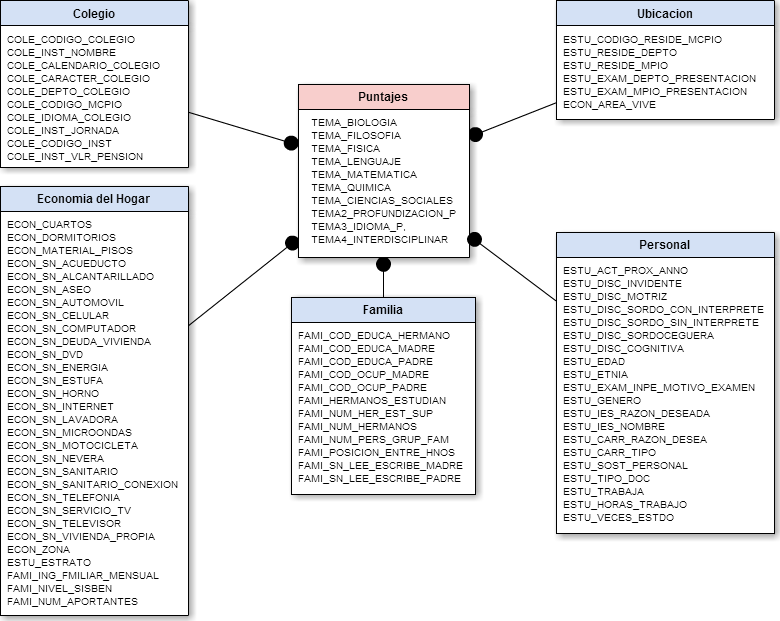
\includegraphics[scale=0.65]{datamart}
\par\end{centering}
\caption{Diseño logico del modelo de almacenamiento de datos.}
\label{fig:figura2}
\end{figure}
En el diseño lógico del modelo dimensional (figura \ref{fig:figura2}) se pueden observar las dimensiones y la tabla de hechos.

Las dimensiones, que contienen los atributos que ayudan a responder las preguntas que se pueden plantear sobre el modelo, constan de la información que define las particularidades de un evaluado. Estas dimensiones son: 
\begin{itemize}
\item \textbf{Colegio}: brinda información sobre el colegio en el que estudia o estudió el evaluado, por ejemplo el carácter, el calendario, la jornada escolar, entre otros.
\item \textbf{Economía del hogar}: brinda información sobre el ambiente económico del evaluado, como por ejemplo las características físicas de su hogar, como el material de los pisos y los sistemas de servicios públicos disponibles en él. Además de informar también sobre los ingresos monetarios y la cantidad de personas en las que deben repartirse estos ingresos.
\item \textbf{Familia}: brinda información sobre las características de la familia del evaluado, como por ejemplo las ocupaciones y niveles educativos de sus padres y hermanos.
\item \textbf{Ubicación}: brinda información sobre la zona geográfica donde vive el evaluado, como el municipio y departamento, y si vive en una zona rural o urbana.
\item \textbf{Personal}: brinda información sobre las características físicas y de personalidad del estudiantes, como su edad, el genero, información sobre discapacidades, las razones que lo llevaron a escoger una carrera, entre otras.
\end{itemize}
Para una mayor información sobre el significado de cada uno de estos atributos y de la forma en cómo se almacenan en las bases de datos, se puede observar el diccionario de datos del ICFES.

En la tabla de hechos, la cual almacena los atributos que contienen la información con la cual se responderá  a las preguntas planteadas al modelo, se pueden observar los registros que indican el puntaje en cada una de las áreas académicas evaluadas. 

Cómo se relacionó en la sección \ref{sec:saber11}, las áreas académicas son 14, 8 de obligatoria presentación para todos los evaluados y 6 áreas electivas de las cuales se debe elegir una. Estas 6 electivas constan de 4 profundizaciones y 2 pruebas interdisciplinares, por eso en los atributos de la tabla hechos se encuentran los atributos  TEMA2_PROFUNDIZACION_P, TEMA4_INTERDISCIPLINAR, estos fueron interpretados con la ayuda de un código que indicaba cual prueba escogió cada evaluado.

Así, con el procesamiento de esta información, que fue recolectada, homogeneizada y almacenada nuevamente, se pudo proceder a trabajar con los distintos algoritmos de clasificación elegidos para evaluar en el trabajo de grado. La descripción del desarrollo de esta etapa de evaluación se encuentra en el siguiente capítulo.